Veamos los siguientes sistemas:


\begin{gather}
    G_1(s) = \frac{34}{s^3 + 11s^2 +44s +34} \quad G_2(s) = \frac{s^3 + 2s^2 + s + 1}{s^4 + s^3 + 8s + 1} \\[0.1cm] 
    G_3(s) = \frac{1}{s^4 + 15s^3 + 100s^2 +250s}
\end{gather}


El siguiente código en MATLAB representa estos 3 sistemas y determina si son estables o no mediante los polos:

\begin{lstlisting}
clc
clear
close all


function estable(num, den)
    G = tf(num, den);
    polos = pole(G);
    parte_real = real(polos);
    if any(parte_real >= 0)
        disp('El sistema es inestable o criticamente estable')
    else    
        disp('El sistema es estable')
    end
end

%Para G1
G1 = tf([34], [1, 11, 44, 34]);
estable([34], [1, 11, 44, 34])
>> El sistema es estable

%Para G2
G2 = tf([1, 2, 1, 1], [1, 1, 0, 8, 1]);
estable([1, 2, 1, 1], [1, 1, 0, 8, 1])
>> El sistema es inestable o criticamente estable

%Para G3
G3 = tf([1], [1, 15, 100, 250, 0]);
estable([1], [1, 15, 100, 250, 0])
>> El sistema es inestable o criticamente estable
\end{lstlisting}




Se observa que los sistemas $G_2$ y $G_3$ son inestables ya que presentan polos positivos o nulos. Para esto, podemos compensar el sistema mediante una constante $k$. Para esto, probaremos distintos valores de $k$ y ver si compensan o no el sistema. En la tabla ... se observa si dicho valor de $k$ es ideal para el sistema


\begin{table}[ht!]
    \centering
    \begin{tabular}{|c|c|c|c|c|}
        \hline
        & $G_1$ & $G_2$ & $G_3$ & Ninguno\\
        \hline
        $k = 204$ & &\checkmark & \checkmark& \\[0.2cm]
        $k = 23$& &\checkmark &\checkmark & \\[0.2cm]
        $k = 0.01$& \checkmark & & \checkmark& \\[0.2cm]
        $k = 0.8$& \checkmark& &\checkmark & \\[0.2cm]
        $k = 5.5$&\checkmark & \checkmark & \checkmark & \\
        \hline
    \end{tabular}
\end{table}


Aunque el cuadro represente cuáles valores de $k$ estabilizan el sistema, el criterio es buscar los polos más a la izquierda y con menor parte imaginaria. Por lo tanto, para $G_1$ es recomendable $k = 0.8$; $G_2$ es recomendable $k = 5.5$ y por último $G_3$ es recomendable $k = 204$.

El siguiente código representa cómo se realizó esto en MATLAB

\begin{lstlisting}
K = [204, 23, 0.01, 0.8, 5.5];
F = [G1, G2, G3];

j = 0;
for f = F
    j = j + 1;
    fprintf('G%g\n', j)
    for k = K
        fprintf('--------------------\n')
        fprintf('k = %g\n', k)
        sis = feedback(f, k);
        polos_sis = pole(sis);
        real_sis = real(polos_sis);
        fprintf('Polos %g\n', real_sis)
        if any(real_sis >= 0)
            continue;
        else
            fprintf('k = %g es ideal para G%g\n', k, j)
        end
    end
end
\end{lstlisting}



Veamos el siguiente sistema:

\begin{equation}
    G(s) = \frac{4}{s(s+2)}
\end{equation}

\noindent Su lugar de raíces y su respuesta escalón está en la figura \ref{fig:4}
\begin{figure}[ht!]
    \centering
    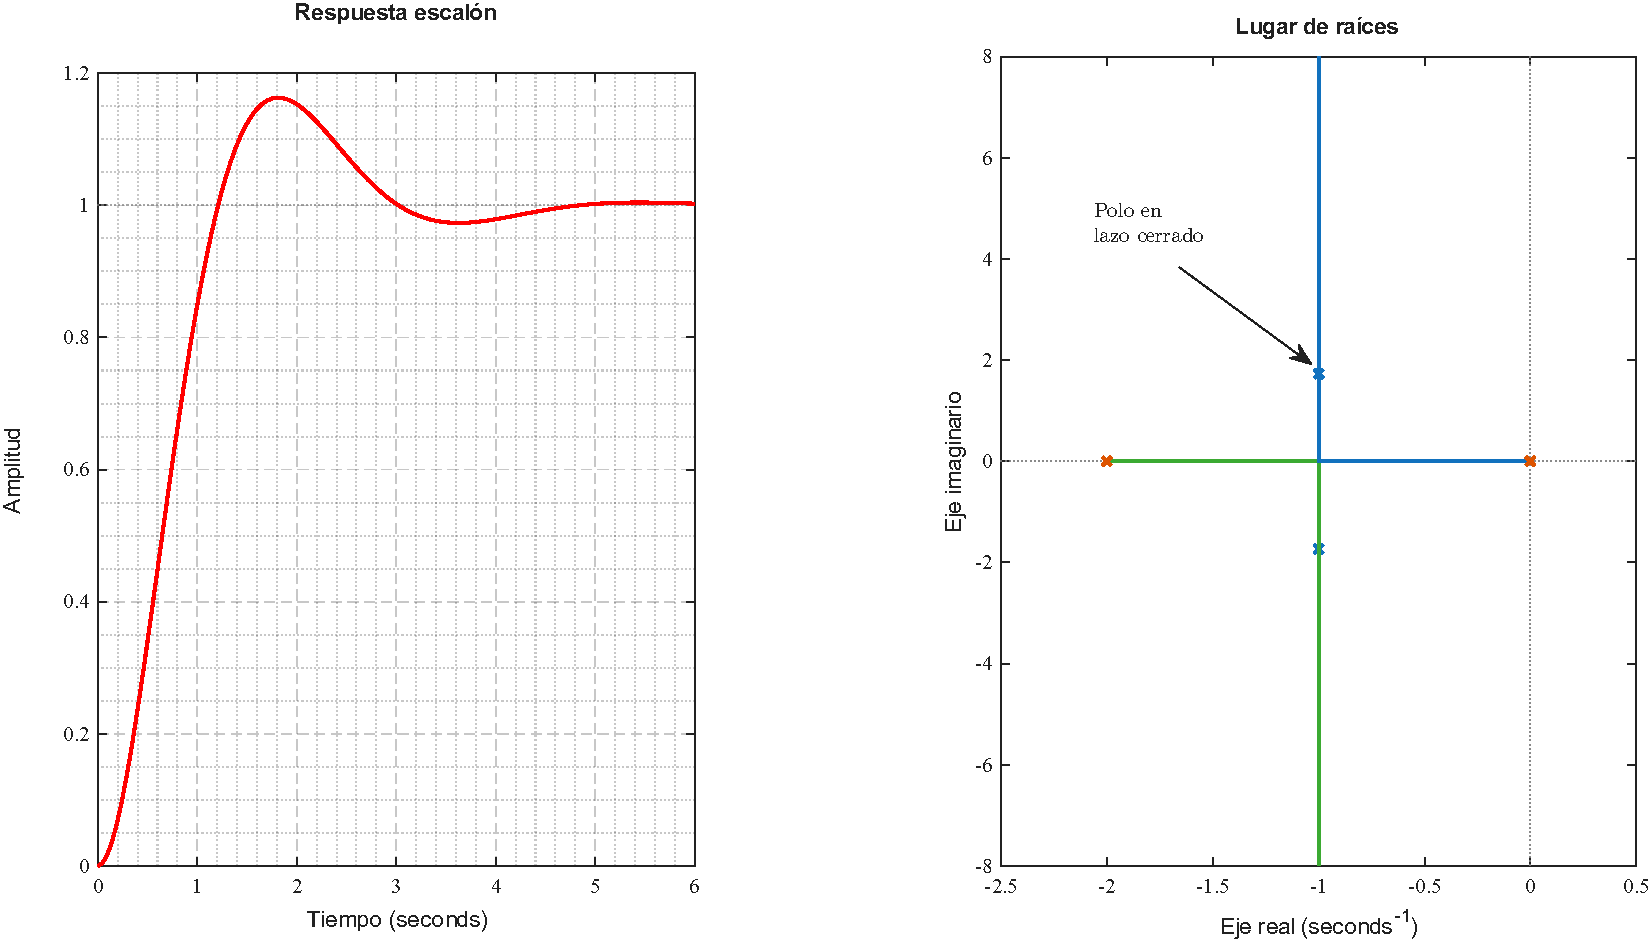
\includegraphics[width=0.95\textwidth]{imagenes/analisis_step_yrootlocus.pdf}
    \caption{Respuesta del sistema $G(s)$ ante una entrada escalón y su lugar de raíces. Se observa que tiene polos en 0 y -2 y $-1 \pm 1.732 i$ para el lazo cerrado. }
    \label{fig:4}
\end{figure}


Ahora, por alguna razón que desconocemos, queremos ubicar los polos en $-2 \pm 2\sqrt{3}i$, por lo que necesitamos un compensador. Para esto empleareamos la siguiente lógica para encontrar un compensador que pase por esos polos.

\begin{tcolorbox}[colback=blue!5!white,colframe=blue!75!black,title=Compensador para $G(s)$, breakable]
Se empleará el cálculo que propone \textit{Katsuhiko Ogata : Ingeniería de Control Moderna}, capítulo 6, sección 6.6. Usaremos un compensador de adelanto. Un compensador de adelanto $H(s)$ tiene la siguiente función de transferencia:

\begin{equation}
    H(s) = K_c \displaystyle\frac{s + \displaystyle\frac{1}{T}}{s + \displaystyle\frac{1}{\alpha T}}
\end{equation}


Para determinar estos valores, determinemos la suma de los ángulos en la localización deseada de uno de los polos dominantes en lazo cerrado con los polos y ceros en lazo abierto del sistema original, determinando el ángulo $\phi$ necesario que va a contribuir al compensador. Por lo tanto:

\begin{equation}
    \phi = 180^{\circ} - 120^{\circ} - 90^{\circ} = -30^{\circ}
\end{equation}

El déficit en el ángulo de $30^{\circ}$ debe estar contribuido por un compensador en adelante. 

Hay varias maneras de obtener la localización del cero y del polo del compensador en adelante. Veamos el siguiente método y para eso analicemos la siguiente figura:

\begin{center}
    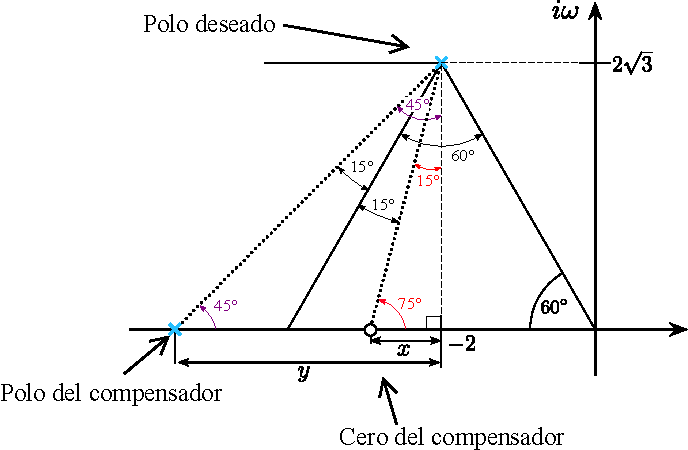
\includegraphics[width=0.8\textwidth]{imagenes/compensador_grafica.pdf}
\end{center}


Dado que el ángulo fue de $30^{\circ}$, entonces ese ángulo se lo divide por 2 y se obtiene (en la bisectriz) dos ángulos de $15^{\circ}$. Para calcular $x$ e $y$ podemos usar la siguiente expresión (se deriva de la figura por trigonometría):

\begin{equation}
    s = \frac{2\sqrt{3}}{\tan \alpha}
\end{equation}


\noindent Donde $\alpha = 75^{\circ}$ y $45^{\circ}$. Por lo tanto:

\begin{align*}
    x = \frac{2\sqrt{3}}{\tan 75} = 0.9282\\[0.2cm]
    y = \frac{2\sqrt{3}}{\tan 45} = 3.4641
\end{align*}

Si ahora a ambas expresiones le sumamos 2 obtenemos el cero y el polo del compensador:

\begin{align*}
    c = x + 2 = 2.9282\\[0.2cm]
    p = y + 2 = 5.4641
\end{align*}


Cabe aclarar que ambos resultados es el valor absoluto. Al estar en el semiplano izquierdo, $c$ y $p$ tienen signo negativo. 

Para calcular $K_c$ se determina a partir de la condición de magnitud:

\begin{equation}
    \left|K_c \frac{s + 2.9282}{s + 5.4641}\frac{4}{s(s + 2)}\right|_{s = -2 + 2\sqrt{3}i} = 1
\end{equation}


Despejando $K_c$ y reemplazando en $s$ por el valor, se obtiene:

\begin{equation*}
    K_c = 4.732
\end{equation*}


Por lo tanto, el compensador es:

\begin{equation}
    H(s) = 4.732\ \frac{s + 2.9282}{s + 5.4641}
\end{equation}


La siguiente figura representa la respuesta del sistema compensado ante una entrada escalón

\begin{center}
    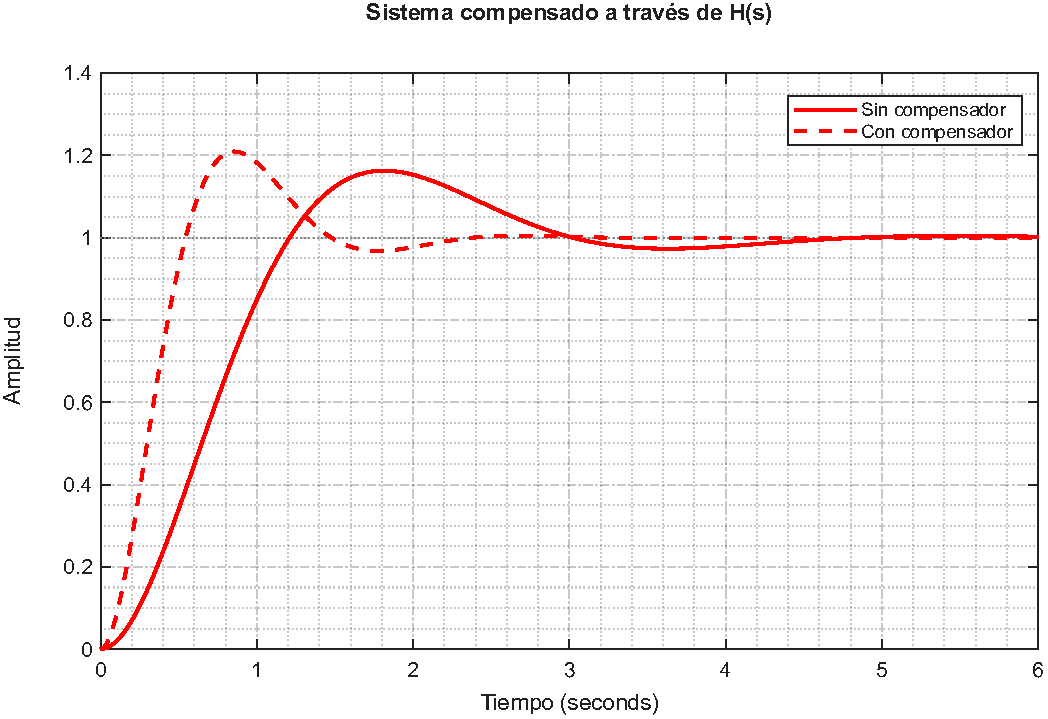
\includegraphics[width=0.8\textwidth]{imagenes/step_compensador.pdf}
\end{center}


Código usado 

\begin{lstlisting}
%El problema sugiere un compensador en serie con realimentacion unitaria
%{
Segun Ogata, la adicion de ceros al sistema hace que el
lugar de raices se desplace a la izquierda, siendo
mas estable el sistema. En cambio, la adicion de polos
lo hace mas inestable (tiende el lugar de raices
a la derecha)
%}
Gs = zpk([], [0, -2], 4);
sist = feedback(Gs, 1);
fig = figure;
theme(fig, 'light');
subplot(1,2,1)
stepplot(sist, 'r')
subplot(1,2,2)
rlocus(sist)
hold on
rlocus(Gs)

%Compensador calculado siguiendo la bibliografia del Ogata
Hs = zpk([-2.9282], [-5.4641], 4.732);
Gs_compensado = feedback(Hs*Gs, 1);
stepplot(sist, 'r')
hold on
stepplot(Gs_compensado, 'r--')
legend('Sin compensador', 'Con compensador')

\end{lstlisting}



\end{tcolorbox}


Por último, se puede usar funciones como \texttt{pidtune} o \texttt{pidtool} para ver cuáles son las funciones compensadores para compensar un sistema $G(s)$. Por ejemplo, para el sistema $G_1(s)$ probamos un compensador proporcional integral y un PID (proporcional, integral y derivativo).

\begin{lstlisting}
parametros_pi = pidtune(G1, 'pi');
>>  
             1 
  Kp + Ki * ---
             s 

  with Kp = 1.85, Ki = 1.86

parametros_pid = pidtune(G1, 'pidf');
>>  
             1            s    
  Kp + Ki * --- + Kd * --------
             s          Tf*s+1 

  with Kp = 1.99, Ki = 2.42, Kd = 0.348, Tf = 0.00494
\end{lstlisting}

